\documentclass{article}
\usepackage{geometry}
\geometry{a4paper, margin=1in}
\usepackage{graphicx}
\usepackage[colorlinks=true, linkcolor=blue, citecolor=blue, urlcolor=blue]{hyperref}
\usepackage{listings}
\usepackage{xcolor}
\usepackage{amsmath}
\usepackage{enumitem}
\usepackage{float}
\usepackage{subcaption}

\lstset{
    language=Python,
    basicstyle=\ttfamily\footnotesize\selectfont, % use the selected monospaced font
    backgroundcolor=\color{white},
    keywordstyle=\color{blue},
    commentstyle=\color{gray},
    stringstyle=\color{red},
    numbers=left,
    numberstyle=\tiny\color{gray},
    stepnumber=1,
    numbersep=10pt,
    frame=single,
    breaklines=true,
    captionpos=b,
    tabsize=4
}

\title{Assignment 1 - Training Random CNNs in Tensorflow \\
\large Who needs activation functions anyway?}
\author{
    [Welby Seely] \\
    \texttt{[wseely@emich.edu]}
}
\date{\today}

\begin{document}

    \maketitle

    \section{Common Hyperparameters}\label{sec:preamble}

    RELU was used for the convolutional activations across all tests, softmax was applied to the output with a couple notable exceptions.
    Used the Adam optimizer for its efficiency in stochastic gradient descent~\cite{kingma2017adammethodstochasticoptimization} and SparseCategoricalCrossentropy because this is a classification problem.
    20 epochs were used for all tests except against the slapdash residual CNN where 50 epoches were used.

    \section{Base Design}\label{sec:base-design}

    As a starting point, I used the base design provided in class for MINST, modified for the CIFAR-10 dataset (32 x 32 images, 3 RGB channels).
    \\
    \begin{lstlisting}[label={lst:base_cnn}]
        model = models.Sequential([
            layers.Conv2D(32, (3, 3), activation='relu', input_shape=(32, 32, 3)),
            layers.MaxPooling2D((2, 2)),
            layers.Conv2D(64, (3, 3), activation='relu'),
            layers.MaxPooling2D((2, 2)),
            layers.Conv2D(64, (3, 3), activation='relu'),
            layers.Flatten(),
            layers.Dense(64, activation='relu'),
            layers.Dense(10, activation='softmax'),
        ])
    \end{lstlisting}

    \begin{itemize}
        \item Accuracy: 70.91\%
        \item Training Time: 21 seconds
    \end{itemize}

    \begin{figure}[!htbp]
        \centerline{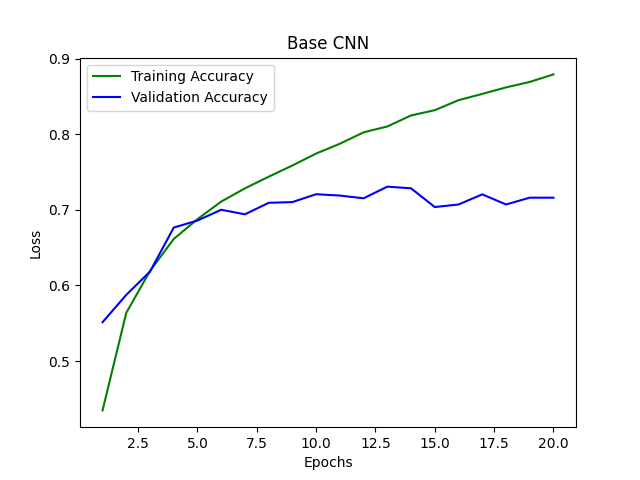
\includegraphics[width=0.55\columnwidth]{Base CNN}}
        \caption{Yay the basic CNN didn't fail in spectacular catastrophe}
        \label{fig:base-cnn}
    \end{figure}

    There were diminishing returns after about 5 epochs.

    Now that the base test is out of the way, I experimented with removing elements to get a better understanding of the characteristics and mechanisms of CNNs.

    \section{Time to Go Monochrome!}\label{sec:one-channel}

    Alright, 70\% accuracy, not bad.
    But how important are the 3 channels to classification?
    Let's find out by testing the same network using only one RGB channel at a time:

    \begin{lstlisting}[label={lst:channel_code}]
        for channel in Channels:
            train_images_filtered = self.filter_rgb_channel(train_images, channel.value)
            test_images_filtered = self.filter_rgb_channel(test_images, channel.value)

            model = models.Sequential([
                layers.Conv2D(32, (3, 3), activation='relu', input_shape=(32, 32, 1)),
                layers.MaxPooling2D((2, 2)),
                layers.Conv2D(64, (3, 3), activation='relu'),
                layers.MaxPooling2D((2, 2)),
                layers.Conv2D(64, (3, 3), activation='relu'),
                layers.Flatten(),
                layers.Dense(64, activation='relu'),
                layers.Dense(10, activation='softmax'),
            ]))
    \end{lstlisting}

    Channels are removed using idiomatic Python list resizing:

    \begin{lstlisting}[label={lst:bye-bye-channel}]

    def filter_rgb_channel(images, channel):
        return images[:, :, :, channel:channel + 1]
    \end{lstlisting}

    The results:

    \begin{itemize}
        \item Red Channel Only
        \begin{itemize}
            \item Accuracy: 0.6731\%
            \item Training Time: 19.56 seconds
        \end{itemize}
        \item Green Channel Only
        \begin{itemize}
            \item Accuracy: 0.6759\%
            \item Training Time: 19.86 seconds
        \end{itemize}
        \item Blue Channel Only
        \begin{itemize}
            \item Accuracy: 0.6801\%
            \item Training Time: 19.90 seconds
        \end{itemize}
    \end{itemize}

    The loss in accuracy wasn't negligible, but a ~2.5\% diff in accuracy is much smaller than I anticipated.
    Training time is comparable to the base model, which I did expect - removing 2 of the 3 channels does not change the number of parameters by an order of magnitude, and the parallelized nature of matrix multiplication on a GPU isn't going to necessarily scale linearly anyway.

    \begin{figure}
        \begin{subfigure}[h]{0.5\linewidth}
            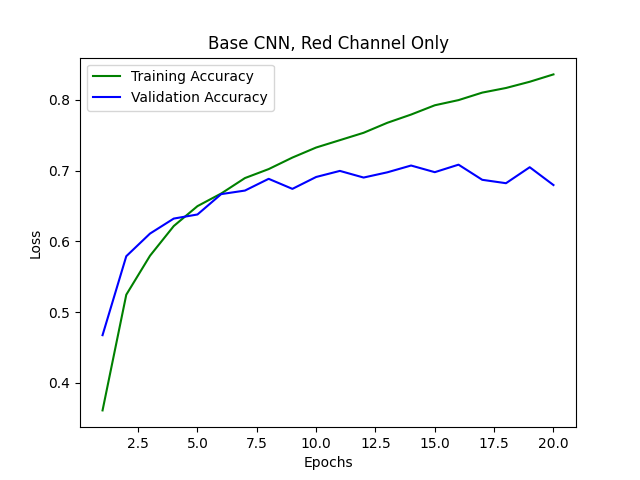
\includegraphics[width=\linewidth]{Base CNN, Red Channel Only}
            \caption{Red Channel}
        \end{subfigure}
        \hfill
        \begin{subfigure}[h]{0.5\linewidth}
            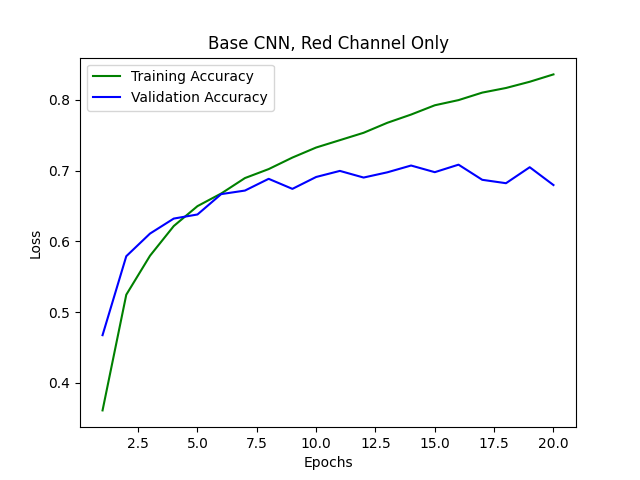
\includegraphics[width=\linewidth]{Base CNN, Red Channel Only}
            \caption{Green Channel}
        \end{subfigure}
        \hfill
        \begin{subfigure}[h]{0.5\linewidth}
            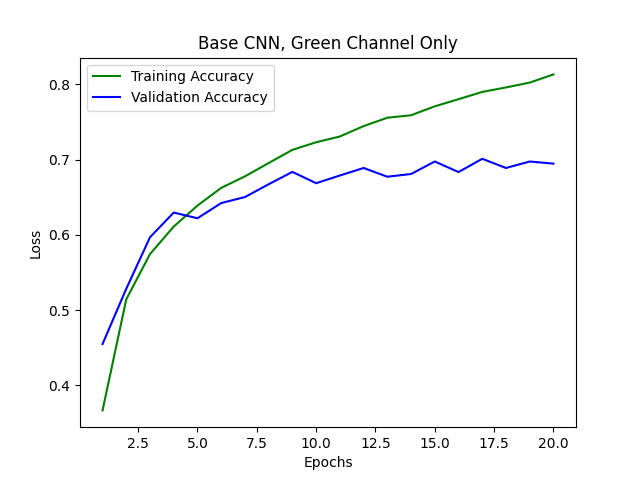
\includegraphics[width=\linewidth]{Base CNN, Green Channel Only}
            \caption{Blue Channel}
        \end{subfigure}\label{fig:figure}%
    \end{figure}

    \section{Removing Activation Functions With Wild Abandon}\label{sec:wild-abandon}

    \subsection{Farewell ReLU, My Beloved!}\label{subsec:farewell-my-beloved-relu!}

    Let's take the base network, and remove ReLUs from the convolutional layers:

    \begin{lstlisting}[label={lst:no_relu}]
        model = models.Sequential([
            layers.Conv2D(32, (3, 3), activation=None, input_shape=(32, 32, 3)),
            layers.MaxPooling2D((2, 2)),
            layers.Conv2D(64, (3, 3), activation=None),
            layers.MaxPooling2D((2, 2)),
            layers.Conv2D(64, (3, 3), activation=None),
            layers.Flatten(),
            layers.Dense(64, activation=None),
            layers.Dense(10, activation='softmax'),
        ])
    \end{lstlisting}

    \begin{itemize}
        \item Accuracy: 62.68\%
        \item Training Time: 20.75 seconds
    \end{itemize}

    \begin{figure}[!htbp]
        \centerline{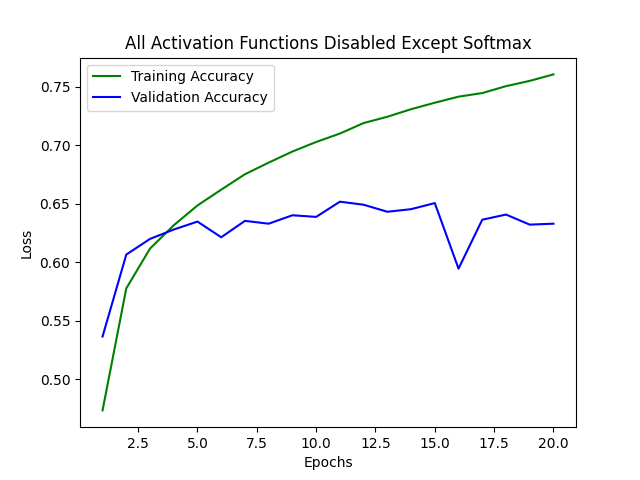
\includegraphics[width=0.55\columnwidth]{All Activation Functions Disabled Except Softmax}}
        \caption{Huh, this isn't entirely terrible}
        \label{fig:softmax-only1}
    \end{figure}

    Removing the activation functions noticeably reduces accuracy by ~7\%, but the accuracy was still higher than I expected.
    The softmax is doing the heavy lifting here.
    Training time is unchanged because the number of matrix multiplications remains identical to the base model, which takes up the bulk of compute.

    \subsection{Pretending to Remove the Softmax}\label{subsec:pretending-to-remove-the-softmax}

    What if we remove the Softmax activation function, but instead enable the Softmax in the Loss Function itself (i.e.\ the loss function takes in raw logits instead of normalized percentages)?

    \begin{lstlisting}[label={lst:no_softmax_jk}]
        model = models.Sequential([
            layers.Conv2D(32, (3, 3), activation=None, input_shape=(32, 32, 3)),
            layers.MaxPooling2D((2, 2)),
            layers.Conv2D(64, (3, 3), activation=None),
            layers.MaxPooling2D((2, 2)),
            layers.Conv2D(64, (3, 3), activation=None),
            layers.Flatten(),
            layers.Dense(64, activation=None),
            layers.Dense(10, activation=None),
        ])

        model.compile(optimizer='adam',
                      loss=SparseCategoricalCrossentropy(from_logits=True),
                      metrics=['accuracy'])
    \end{lstlisting}

    \begin{itemize}
        \item Accuracy: 63.39\%
        \item Training Time: 20.81 seconds
    \end{itemize}

    \begin{figure}[!htbp]
        \centerline{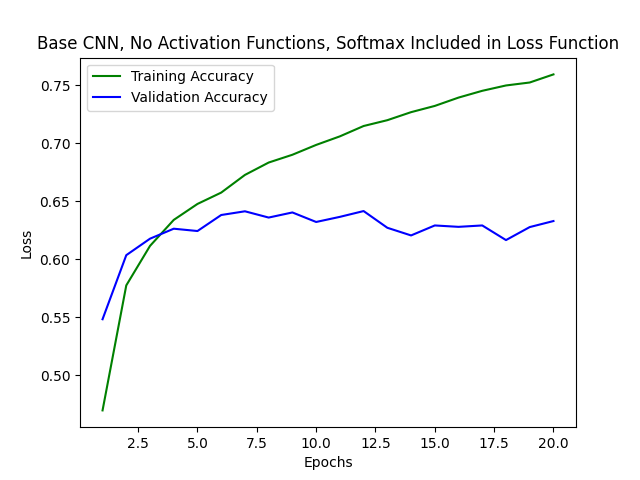
\includegraphics[width=0.55\columnwidth]{Base CNN, No Activation Functions, Softmax Included in Loss Function}}
        \caption{Results are the same as the Softmax-only CNN}
        \label{fig:sneaky-softmax}
    \end{figure}

    Unsurprisingly, the accuracy and training time are basically identical.
    The Softmax applied as a part of the loss function acts as a de-facto activation function.
    There may be mathematical implications on fusing the activation function with the loss function, but in this case the results are identical.

    \subsection{No activation functions at all}\label{subsec:no-activation-functions-at-all}

    Finally, let's remove all activation functions, including the softmax (explicit or implicit):

    \begin{lstlisting}[label={lst:no_activations}]
        model = models.Sequential([
            layers.Conv2D(32, (3, 3), activation=None, input_shape=(32, 32, 3)),
            layers.MaxPooling2D((2, 2)),
            layers.Conv2D(64, (3, 3), activation=None),
            layers.MaxPooling2D((2, 2)),
            layers.Conv2D(64, (3, 3), activation=None),
            layers.Flatten(),
            layers.Dense(64, activation=None),
            layers.Dense(10, activation=None),
        ])

        model.compile(optimizer='adam',
                      loss=SparseCategoricalCrossentropy(from_logits=False),
                      metrics=['accuracy'])
    \end{lstlisting}

    \begin{itemize}
        \item Accuracy: 10.00\%
        \item Training Time: 20.81 seconds
    \end{itemize}

    \begin{figure}[!htbp]
        \centerline{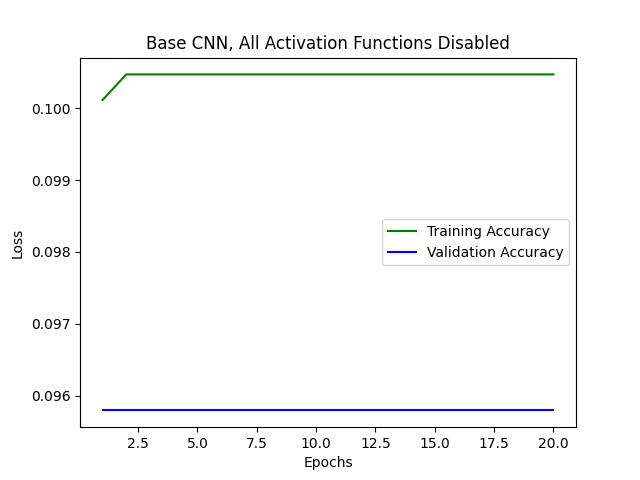
\includegraphics[width=0.55\columnwidth]{Base CNN, All Activation Functions Disabled}}
        \caption{10 classes, equal chance of choosing one of them}
        \label{fig:no-acts}
    \end{figure}

    Without activation functions, the linearly combined matrices have no way of reaching the solution vector space.
    A 10 percent accuracy means that you have an equally random chance at of correctly classifying an image, a heavily parameterized 10-sided die.
    \\
    Training time remains the same because the parameters have remained the same.

    \section{Wait, are the Convolutional Layers Important?}\label{cnn-important}

    Removing all activation functions but the softmax produces ok-ish results, what if remove the convolutional layers entirely?

    \begin{lstlisting}[label={lst:just softmax}]
        model = models.Sequential([
            layers.Flatten(),
            layers.Dense(10, activation='softmax'),
        ])
    \end{lstlisting}

    \begin{itemize}
        \item Accuracy: 37.28\%
        \item Training Time: 16.20 seconds
    \end{itemize}

    \begin{figure}[!htbp]
        \centerline{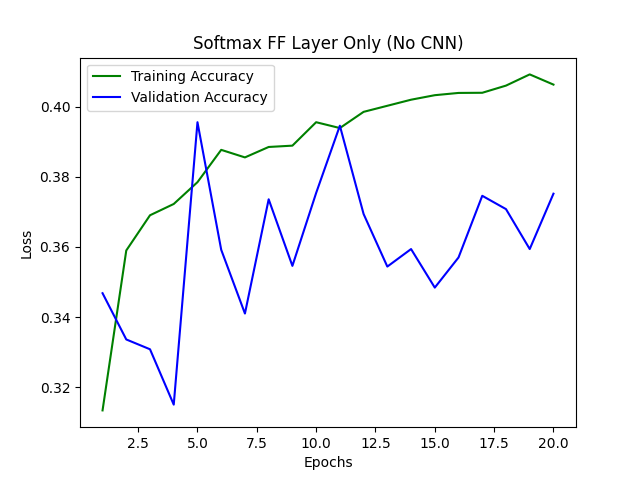
\includegraphics[width=0.55\columnwidth]{Softmax FF Layer Only (No CNN)}}
        \caption{Ok, yeah, the convolutional layers are important}
        \label{fig:ya-important}
    \end{figure}

    We dropped from about 64\% to 37\%.
    Even without activation functions, the convolutional layers contribute significantly to both accuracy and numerical stability.


    \section{Ok Let's Get That Accuracy to at Least 80\%}\label{skip-connections}

    I set a goal for myself to achieve at least 80\% accuracy.
    Playing with kernel size, stride, number of filters, and number of layers was not achieving beyond 74\% accuracy.
    So, I decided to take a look at how Resnet50 is implemented~\cite{mukherjee2022annotated}, and I plopped three skip blocks into the network.

    \begin{lstlisting}[label={lst:bigger}]
        class ResCnn(ModelRunner):

            @staticmethod
            def build_res_block(preceding_layers):
                block = layers.Conv2D(128, (1, 1),  padding='valid')(preceding_layers)
                block = layers.BatchNormalization()(block)
                block = layers.ReLU()(block)
                block = layers.Conv2D(128, (3, 3), padding='same')(block)
                block = layers.BatchNormalization()(block)
                block = layers.ReLU()(block)
                block = layers.Conv2D(256, (1, 1),  padding='valid')(block)
                block = layers.BatchNormalization()(block)
                block = layers.Add()([block, preceding_layers]) # res/skip connection
                return layers.ReLU()(block)

            def run_test(self):
                epoch_count = 50
                test_name = "CNN With Haphazardly Placed Residual Blocks"

                cifar10 = datasets.cifar10
                (train_images, train_labels), (test_images, test_labels) = cifar10.load_data()
                inputs = Input(shape=(32, 32, 3))
                outputs = layers.ZeroPadding2D(padding=(3, 3))(inputs)
                outputs = layers.Conv2D(256, (3, 3), activation='relu', padding='valid')(outputs)
                outputs = layers.MaxPooling2D((2, 2))(outputs)
                outputs = self.build_res_block(outputs)
                outputs = self.build_res_block(outputs)
                outputs = self.build_res_block(outputs)
                outputs = layers.AvgPool2D((2, 2))(outputs)
                outputs = layers.Flatten()(outputs)
                outputs = layers.Dense(512, activation='relu')(outputs)
                outputs= layers.Dense(10, activation='softmax')(outputs)
                model = Model(inputs, outputs)

                model.compile(optimizer=keras.optimizers.Adam(learning_rate=0.0003),
                              loss=SparseCategoricalCrossentropy(from_logits=False),
                              metrics=['accuracy'])
                self._train_model(model, train_images, train_labels, test_images, test_labels, epoch_count, test_name,
                                  show_graph=True)
    \end{lstlisting}

    The network starts off with padding, a conv layer, and a max pooling layer just like the CNN that preceeded it.
    Three ``Residual Blocks'' follow.
    Each residual block contains:

    \begin{itemize}
      \item A Convolution layer that downsamples the channels/filters to 128.
      \begin{itemize}
          \item When down or upsampling, a kernel size of 1 x 1 is used to keep the feature map the same size ~\cite{mukherjee2022annotated}.
      \end{itemize}
      \item A Batch Normalization Layer
      \begin{itemize}
          \item This is used ~\cite{mukherjee2022annotated}.
      \end{itemize}
    \end{itemize}

    \begin{itemize}
        \item Accuracy: 73.48\%
        \item Training Time: 36.41 seconds
    \end{itemize}

    \begin{figure}[!htbp]
        \centerline{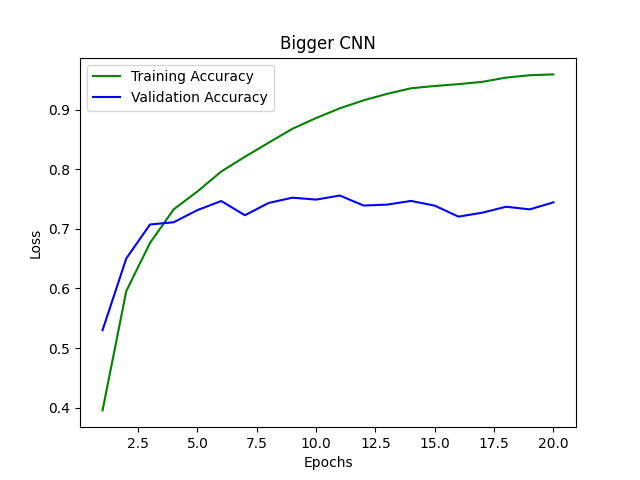
\includegraphics[width=0.55\columnwidth]{Bigger CNN}}
        \caption{Bigger and slightly more accurate CNN}
        \label{fig:bigger}
    \end{figure}

    We bumped up the accuracy from ~70\% to ~74\% which is a decent uplift.
    Training time was almost doubled because of the quadrupling of parameters (122,570 parameters \rightarrow 551,882 parameters).



    \bibliographystyle{plainurl}
    \bibliography{bibliography}
\end{document}
